\section{System Requirements}

\subsection{Customer Requirements}
The system will be a web interface that allows linkback checking, it should be able to handle several "projects" where the links will be listed and show it's status.

\begin{figure}[ht!]
	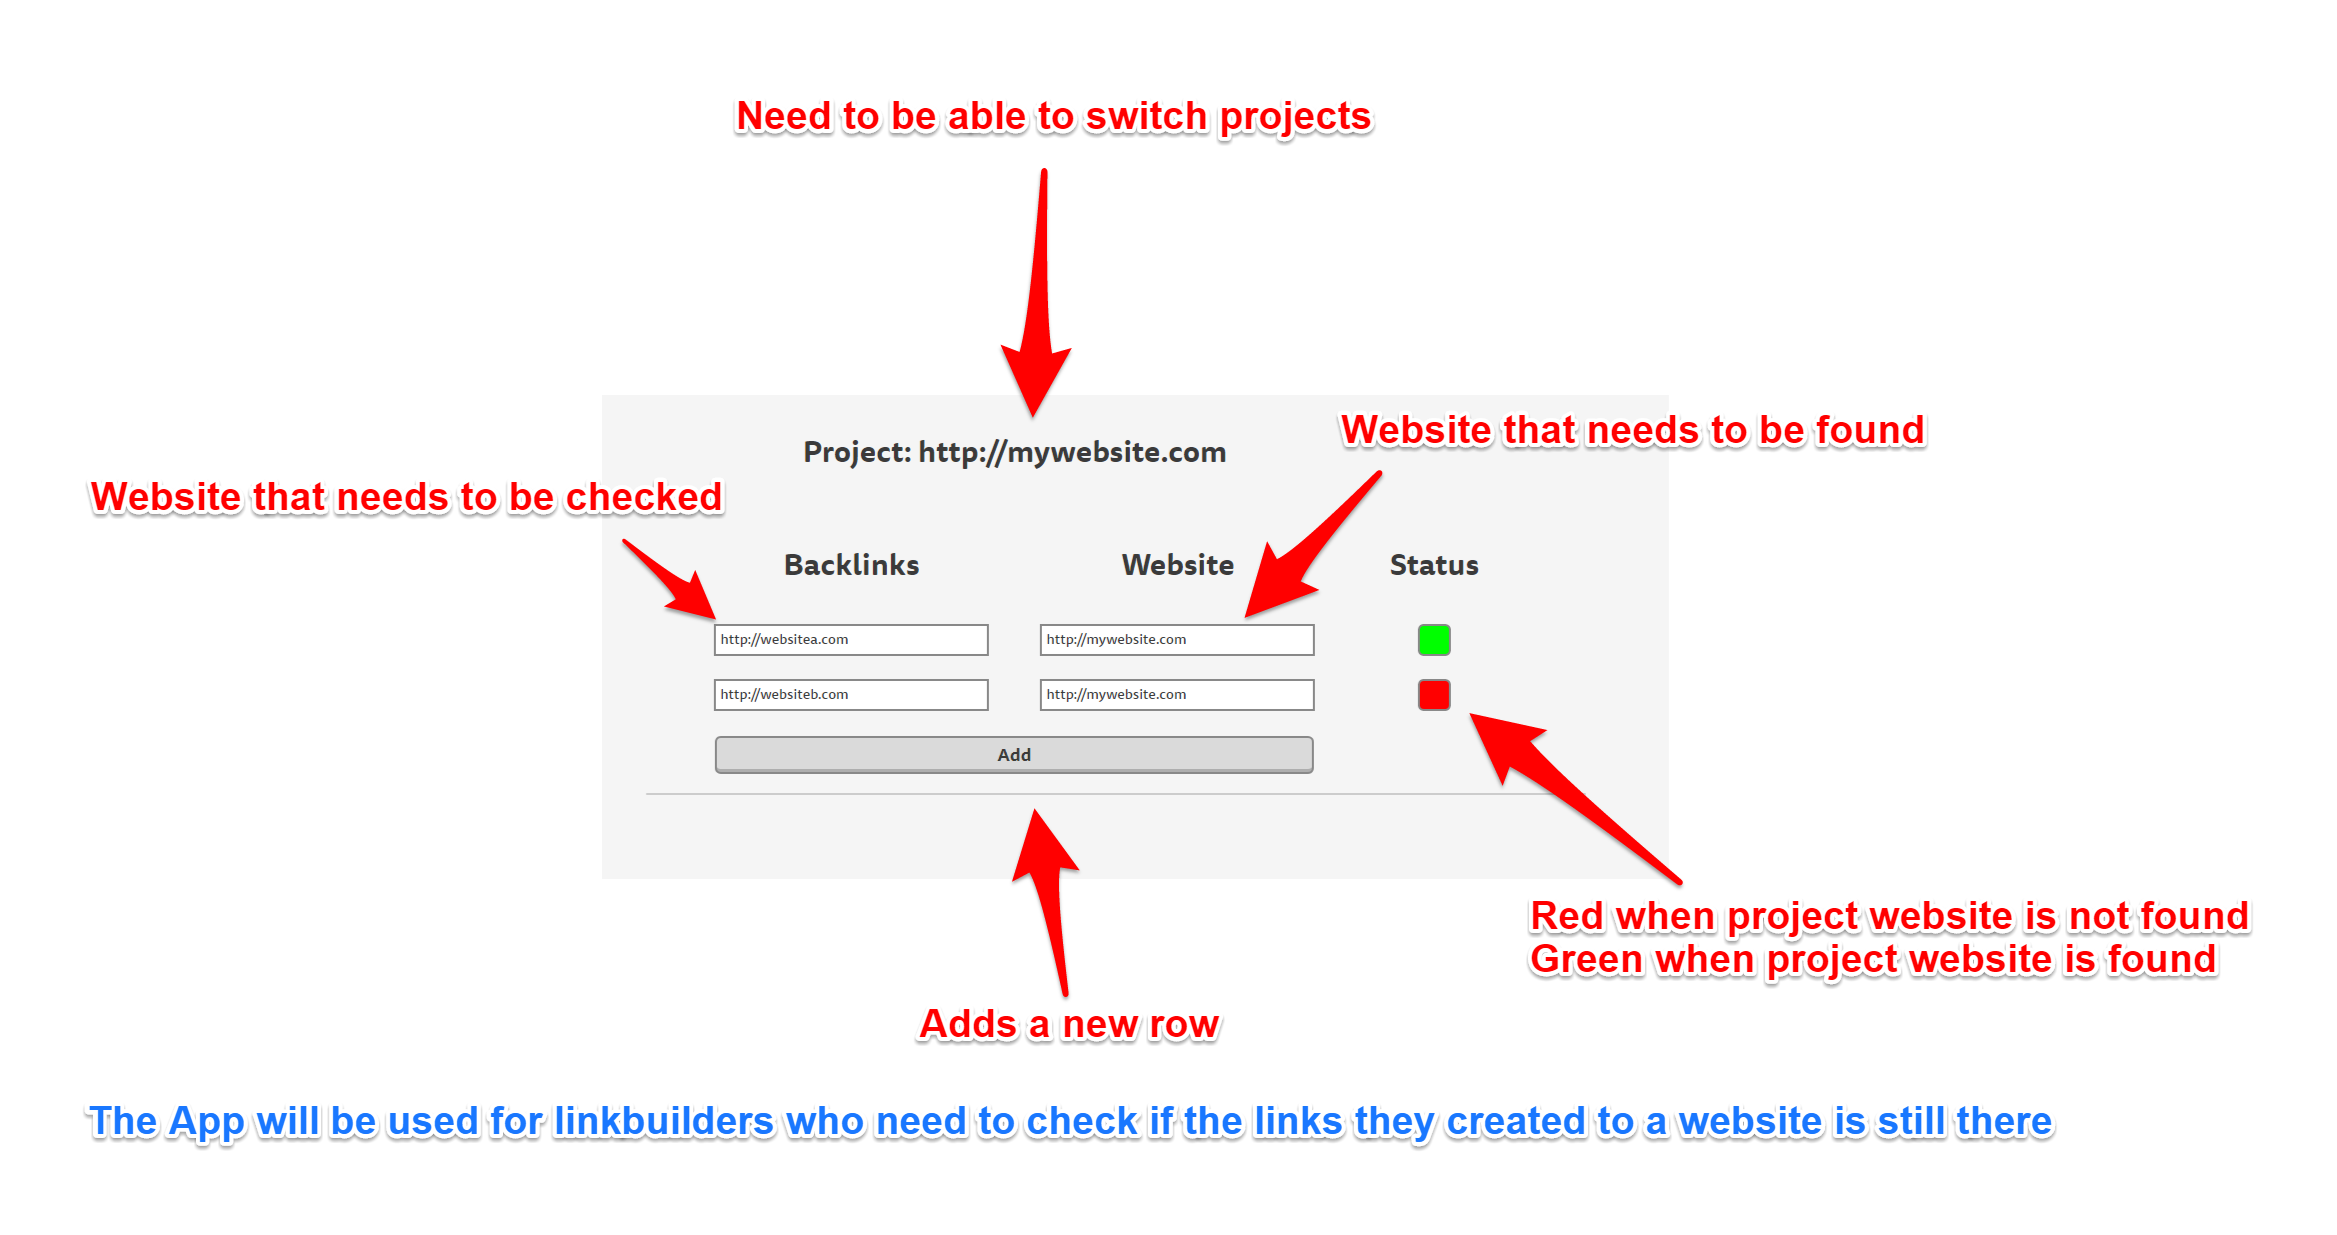
\includegraphics[width=\textwidth]{images/backlinkappfiverrexplained}
	\caption{User provided details}
\end{figure}

\subsection{Requirement Analysis and elicitation}
The following table lists the user requirements from the original system request.
\begin{enumerate}
	\item The system shall allow the unique user identification
	\item The system shall ask for username and password to access it
	\item The system shall identify a special user as administrator who will be able to
	\begin{enumerate}
		\item Add other users to the system.
		\item Permanently delete objects from the system.
		\item recover user deleted items.
		\item block users from login in.
		\item Unblock the users blocked.
	\end{enumerate}
	\item The system shall allow to list, create, modify and delete ''projects'' to group link checker items.
	\item The system shall allow to list, create, modify and delete ''link checker'' items.
	\item The system shall check the link status automatically when displaying the checker list
	\item The system must be developed in PHP
	\item The system could be developed using the Laravel framework.
	\item The system will have an admin template in use for it's display.
\end{enumerate}

\section{System Design}

\subsection{Entity Relationship Diagram}
Please refer to figure \ref{fig:er}
\begin{figure}[ht!]
	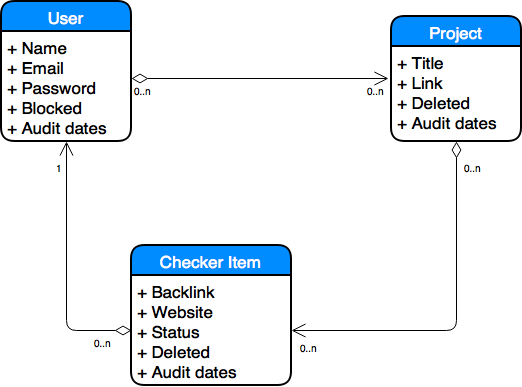
\includegraphics[width=\textwidth]{images/Entity-relationship-diagram-Linkchecker}
	\caption{System Entities and Relationships}
	\label{fig:er}
\end{figure}
\subsection{Use Cases}
Please see figure \ref{fig:uc}
\begin{figure}[ht!]
	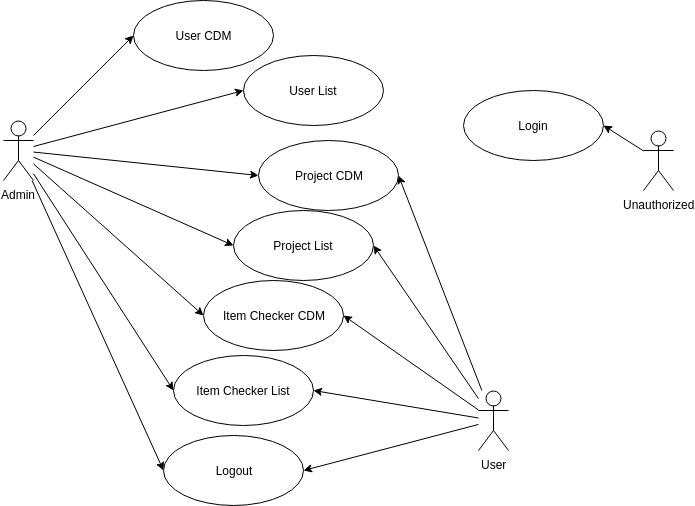
\includegraphics[width=\textwidth]{images/Use-Cases-Linkchecker}
	\caption{System use cases}
	\label{fig:uc}
\end{figure}

\subsection{Design desitions}
\begin{itemize}
	\item The link checker items list will be paged
	\item The link checker items page will have 15 items by default, 25 as a second option and 50 as the last one.
	\item The Angular library will be used for the interface wherever it applies.
\end{itemize}

\subsection{Possible future features}
After doing the requirements analysis, we've come to a list of possible future/extension features which we list below:
\begin{itemize}
	\item Groups/companies.
	\item Distinguished user as manager for a group/company.
	\item New low user level with less permission and under a manager's group/company.
	\item Managers are the only users able to create projects and assign users to it.
	\item low users can only create links on their assigned project.
\end{itemize}

This features can be accommodated in a new project if needed.